\documentclass[a4paper, 11pt]{article}
\usepackage{covington}
\usepackage{amssymb}
\usepackage{amsmath}
\usepackage[catalan]{babel}
\usepackage{graphicx}
\usepackage{eurosym}
\usepackage{subcaption}
\textheight=23.94cm 
\textwidth=17cm 
\topmargin=-1cm 
\oddsidemargin=-0.5cm 
 
\newcommand{\header}[4]{
	\begin{center}
		\rule{\linewidth}{0.5pt}
		
		{\small{#1}}
      
        \vspace{0.2in}
        
		{\large{#2}}
		
        \vspace{0.2in}
        
		{\small{#3}}
		
		\vspace{0.15in}
		
		{#4}
		
		\vspace{-0.1in}
		\rule{\linewidth}{0.6pt}
	\end{center}
}

\begin{document}
 
\header{\sc Barcelona Graduate School of Economics \hfill Master's Degree in Data Science}{\bf Statistical Modeling and Inference $-$ Problem Set \#3}{\sc Niti Mishra $\cdot$ Miquel Torrens $\cdot$ B\'alint V\'an}{October 26\textsuperscript{th}, 2015}
Solution to proposed exercises.\\
% EXERCISE 1
\newline \textbf{\underline{Exercise 1}}\\
\newline \underline{Part 1}\\
\newline The exercise requires two extra parameters not defined, which are $\delta$ and $g$.\\
\newline We keep $\delta$ as the degree of freedom. We will try to find $g$ in the following manner:
\begin{itemize}
\item To start, we compute the sample variance of the model with only the intercept.
\item We plug the result in out first Bayesian iteration as a proxy for $g$, given a specific $\delta$.
\item We obtain an updated result on $g$ after running the model and we use this result to re-run the model  trying to find an updated $g$.
\item We keep running models using this updating method until we detect that $g$ stabilizes, keeping that stable $g$ for the ultimate model.
\end{itemize}
The model shall look as follows:\\
\begin{center}
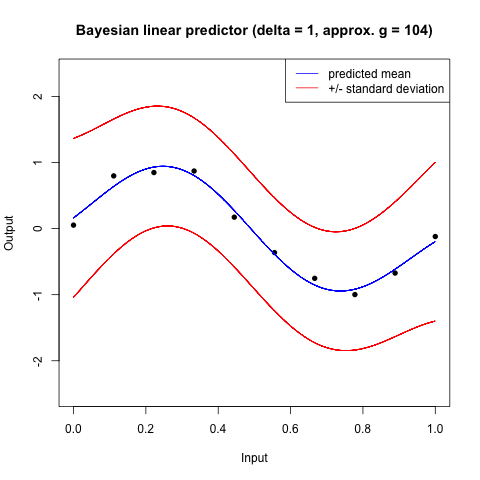
\includegraphics[scale=0.6]{ps3F_plot1.png}
\end{center}
For clarity we will plot the results of posterior draws using $\delta=2$, as used in previous exercises, since it is the value that best suits the data (see lectures).\\
\begin{figure}
\begin{subfigure}{.5\textwidth}
  \centering
  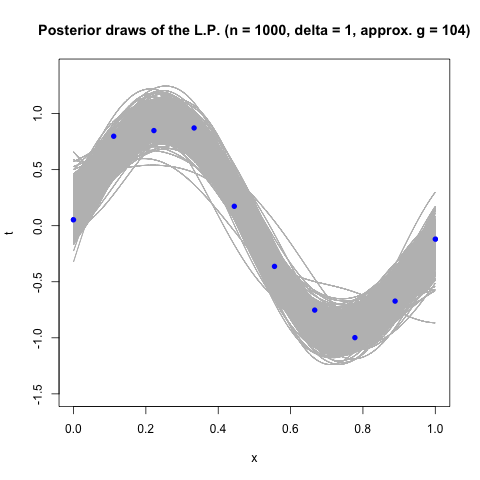
\includegraphics[width=.8\linewidth]{ps3F_plot2.png}
\end{subfigure}
\begin{subfigure}{.5\textwidth}
  \centering
  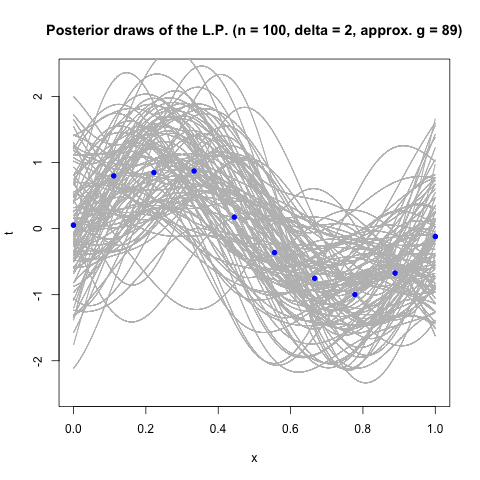
\includegraphics[width=.8\linewidth]{ps3F_plot2_0.png}
\end{subfigure}
\end{figure}
%\begin{center}
%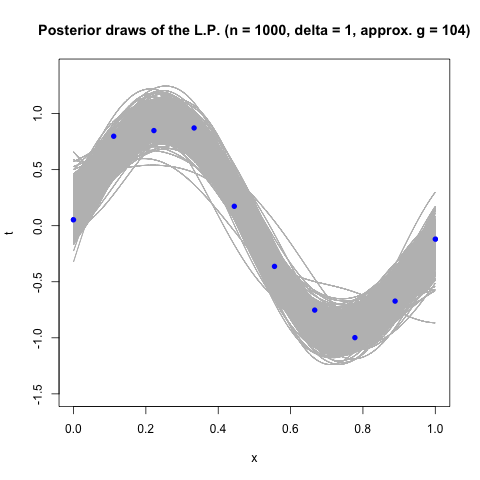
\includegraphics[scale=0.6]{ps3F_plot2.png}
%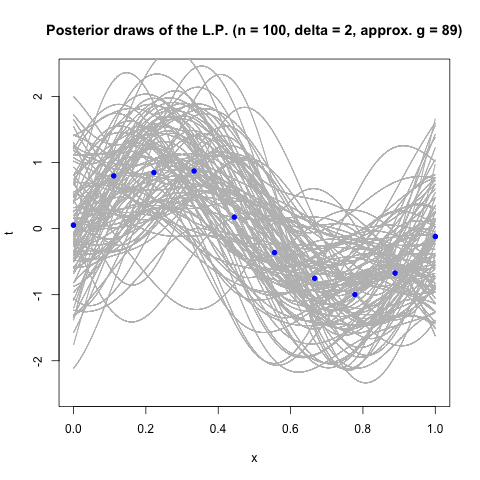
\includegraphics[scale=0.6]{ps3F_plot2_0.png}
%\end{center}
\underline{Part 2}\\
\newline Now we explore how the models are sensible to $\delta$. Note that we fix the value of $\delta$ and that $g$ is then determined by the aforementioned algorithm:\\
\begin{center}
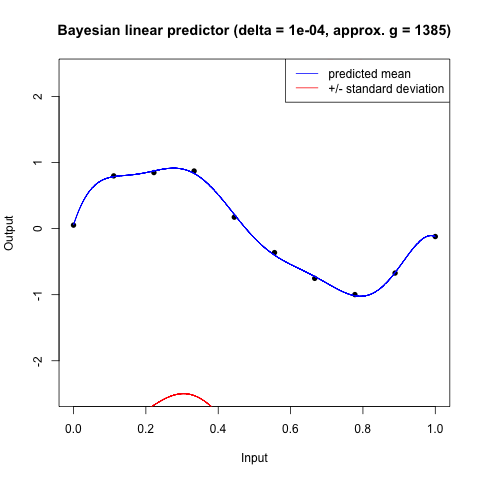
\includegraphics[scale=0.6]{ps3F_plot3_1.png}
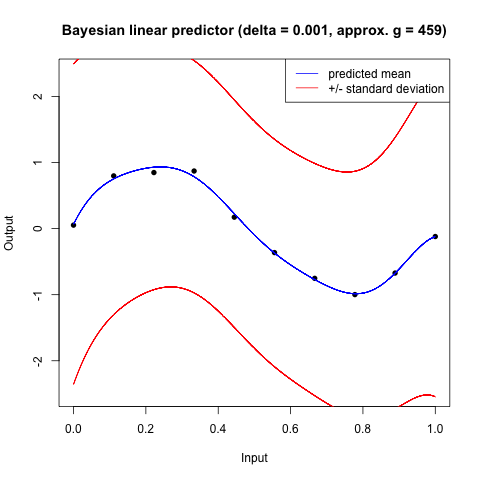
\includegraphics[scale=0.6]{ps3F_plot3_2.png}
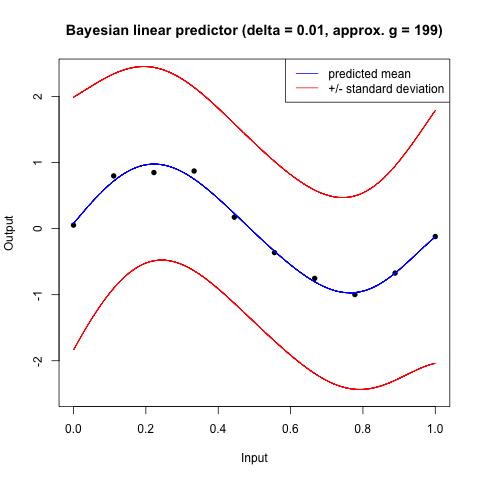
\includegraphics[scale=0.6]{ps3F_plot3_3.png}
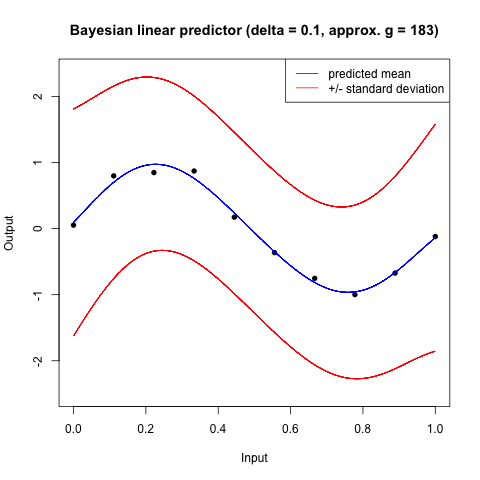
\includegraphics[scale=0.6]{ps3F_plot3_4.png}
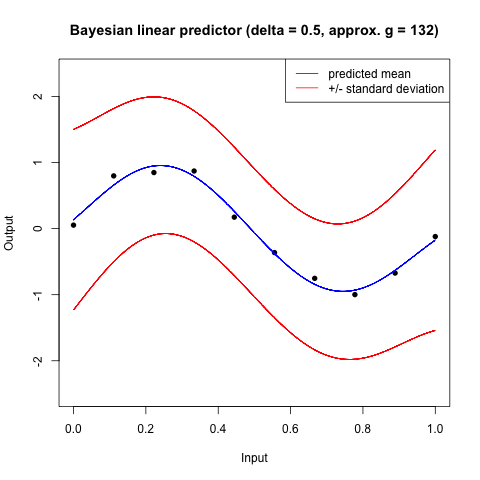
\includegraphics[scale=0.6]{ps3F_plot3.png}
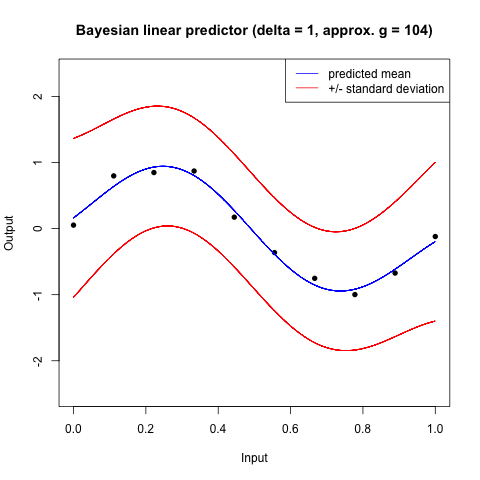
\includegraphics[scale=0.6]{ps3F_plot4.png}
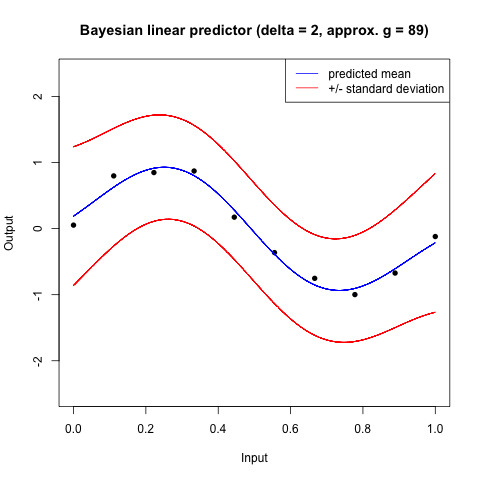
\includegraphics[scale=0.6]{ps3F_plot5.png}
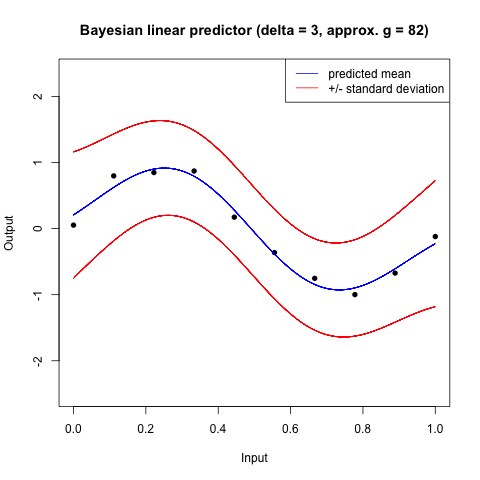
\includegraphics[scale=0.6]{ps3F_plot6.png}
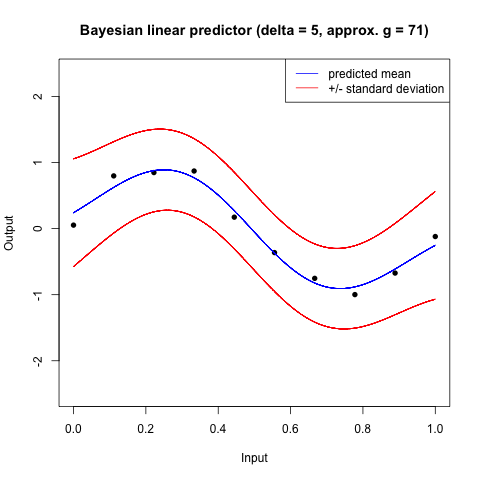
\includegraphics[scale=0.6]{ps3F_plot7.png}
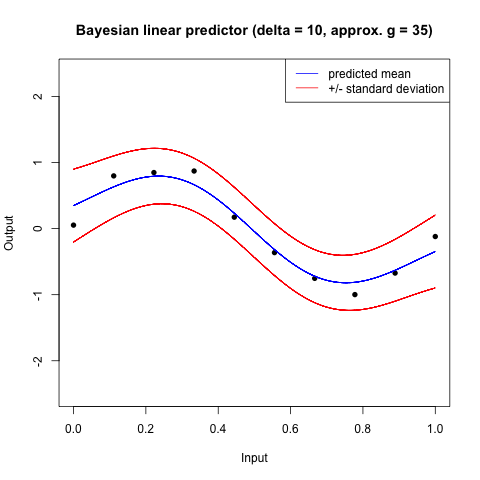
\includegraphics[scale=0.6]{ps3F_plot8.png}
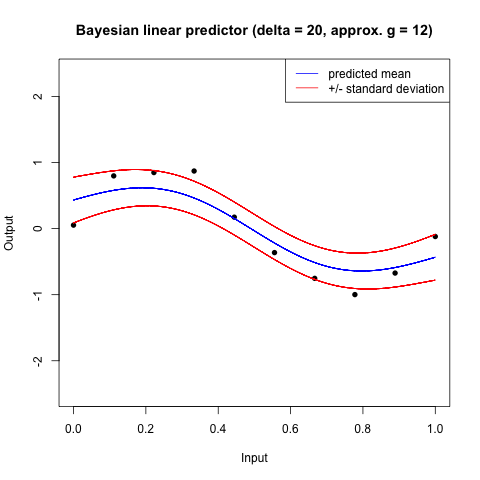
\includegraphics[scale=0.6]{ps3F_plot9.png}
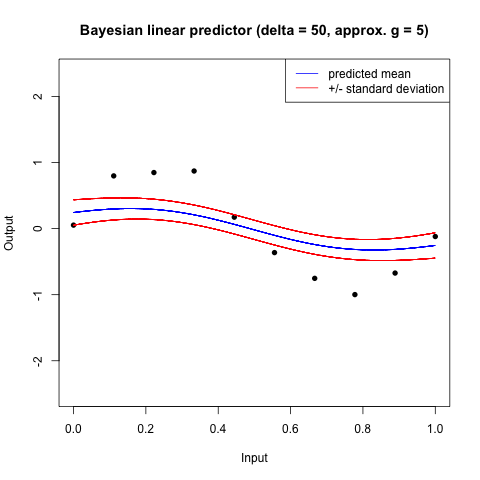
\includegraphics[scale=0.6]{ps3F_plot10.png}
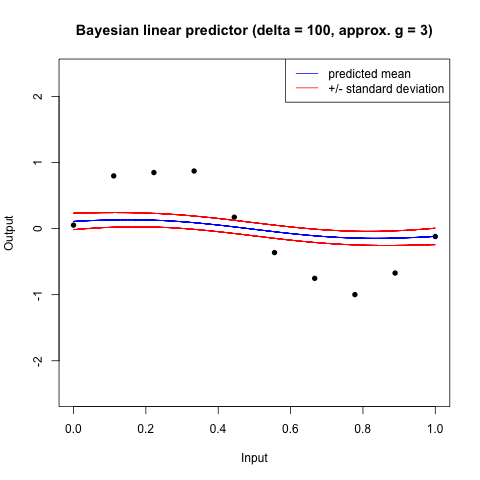
\includegraphics[scale=0.6]{ps3F_plot11.png}
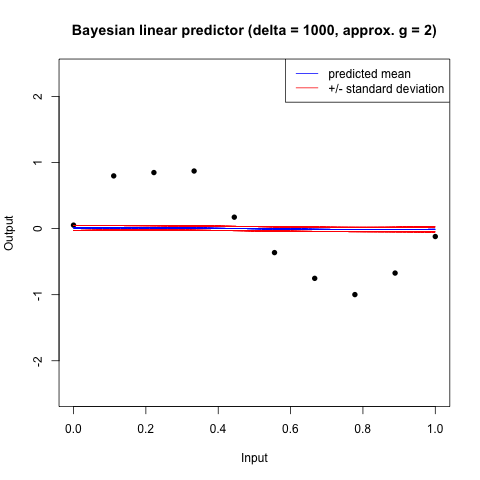
\includegraphics[scale=0.6]{ps3F_plot12.png}
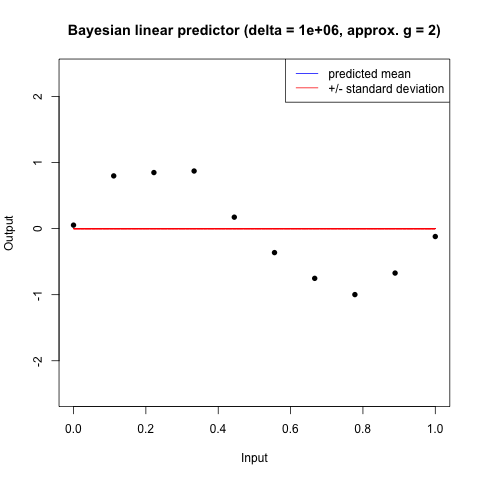
\includegraphics[scale=0.6]{ps3F_plot13.png}
\end{center}
Note that as $\delta$ increases (and $g$ decreases), the prediction becomes flatter and errors become bigger, with a .\\
% EXERCISE 2
\newpage
\textbf{\underline{Exercise 2}}\\
\newline \underline{Part 1}\\
\newline We minimize the function:
\begin{eqnarray}
f(\mu) = (\mu - a)^2 + \lambda |\mu| \nonumber
\end{eqnarray}
Given $a, \lambda > 0$ on $\mu^+$. Hence,
\begin{eqnarray}
\frac{\partial f(\mu)}{\partial \mu^+} = 0 &\Leftrightarrow& 2(\mu^+ -a) + \lambda = 0 \nonumber \\
&\Leftrightarrow& \mu = \left( a - \frac{\lambda}{2} \right)^+ \nonumber
\end{eqnarray}
Also, $f''(\mu^+) = 2$ so this is indeed a minimum.\\
\newline \underline{Part 2}\\
\newline The solution is the following:
\begin{eqnarray}
w_{MAP} &=& \arg \max \log p(\mathbf{w} |  \mathbf{t}) \nonumber \\
&=& \arg \max \log p(\mathbf{t} | \mathbf{w}) + \log p(\mathbf{w}) \nonumber \\
&=& \arg \max \log \prod_{n} p(\mathbf{t}_n | \mathbf{w}) + \log \exp \left\lbrace -\frac{\delta}{2} \sum_i |w_i|  \right\rbrace \nonumber \\
&=&  \arg \max \sum_{n} \log \mathcal{N}(\mathbf{w} | q^{-1} \mathbf{I}) + \log \exp \left\lbrace -\frac{\delta}{2} \sum_i |w_i|  \right\rbrace\nonumber \\
&=& \arg \max \sum_{n} \log \exp \left\lbrace -\frac{1}{2} (\mathbf{t}_n - \mathbf{w})^T q (\mathbf{t}_n - \mathbf{w}) \right\rbrace + \log \exp \left\lbrace -\frac{\delta}{2} \sum_i |w_i|  \right\rbrace + C \nonumber \\
&=& \arg \max \sum_{n} -\frac{1}{2} (\mathbf{t}_n - \mathbf{w})^T q (\mathbf{t}_n - \mathbf{w}) -\frac{\delta}{2} \sum_i |w_i| + C \nonumber \\
&=& \arg \min \sum_{n} q (\mathbf{t}_n - \mathbf{w})^T (\mathbf{t}_n - \mathbf{w}) + \delta \sum_i |w_i| + C \nonumber \\
&=& \arg \min q \sum_{n} \sum_{i} (t_{ni} - w_i)^2 + \delta \sum_i |w_i| + C \nonumber
\end{eqnarray}
We now we maximize this expression with respect to $w_i$:
\begin{eqnarray}
\frac{\partial}{\partial w_{i}} = 0 &\Leftrightarrow& -2 q \sum_{n} (t_{ni} - w_{i}) + \delta \frac{w_i}{|w_i|} = 0 \nonumber
\end{eqnarray}
Given that we are working on the side of $w_{i}^{+}$ this simplifies to:
\begin{eqnarray}
\frac{\partial}{\partial w_{i}^{+}} = 0 &\Leftrightarrow& -2 q \sum_{n} (t_{ni} - w_{i}) + \delta = 0  \nonumber \\
&\Leftrightarrow&w_{MAP} = \frac{1}{N} \left( \sum_n t_{ni} - \frac{\delta}{2} q^{-1} \right)^+ \nonumber
%&\Leftrightarrow&w_i = \frac{1}{N} \left( \sum_n t_{ni} - 2\frac{\delta}{q} \right)^+ \nonumber
\end{eqnarray}
\end{document}





